\chapter {Выполнение работы}
\section{Краткое описание проекта}

Проект: создание собственной Internet-компании <<с нуля>>. Команда молодых начинающих разработчиков во главе с опытным ведущим программистом ориентирована на обучение персонала технологиям создания web-сайтов и разработку представительских и корпоративного сайтов. Масштаб проекта: команда из 7 человек, длительность не более 3 месяцев, бюджет не более 650 тыс. руб. Вариант №1.

\section{Задания 1--5}

Дата начала проекта~---~первый понедельник 2-го квартала 2026 года (06.04.2026). Длительность~---~в днях, объём работ~---~в часах, тип задач по умолчанию~---~с фиксированными трудозатратами. Стандартный календарь: рабочие дни Пн--Пт, с 9:00 до 18:00, обед с 13:00 до 14:00. Праздничные дни учтены.

Введены задачи согласно варианту, задачи 1, 7 и 13 являются вехами. Задачи 5--6 являются подзадачами задачи 4, задачи 9~--~12~---~подзадачами задачи 8. Установлены связи между задачами. Создан список ресурсов. Созданные задачи и список ресурсов представлены на рисунках~\ref{fig:1} и~\ref{fig:2}.

\begin{figure}[H]
	\centering
	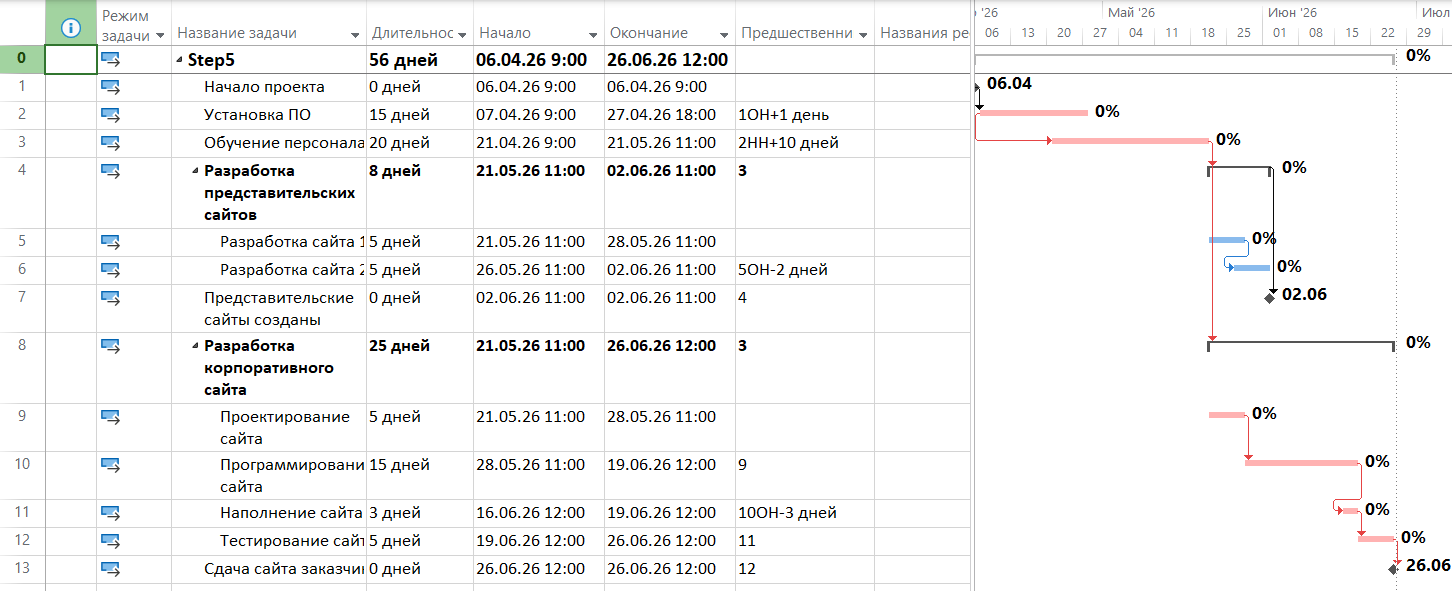
\includegraphics[width=\linewidth]{images/1.png}
	\caption{Список задач после группировки и установления связей}
	\label{fig:1}
\end{figure}

\begin{figure}[H]
	\centering
	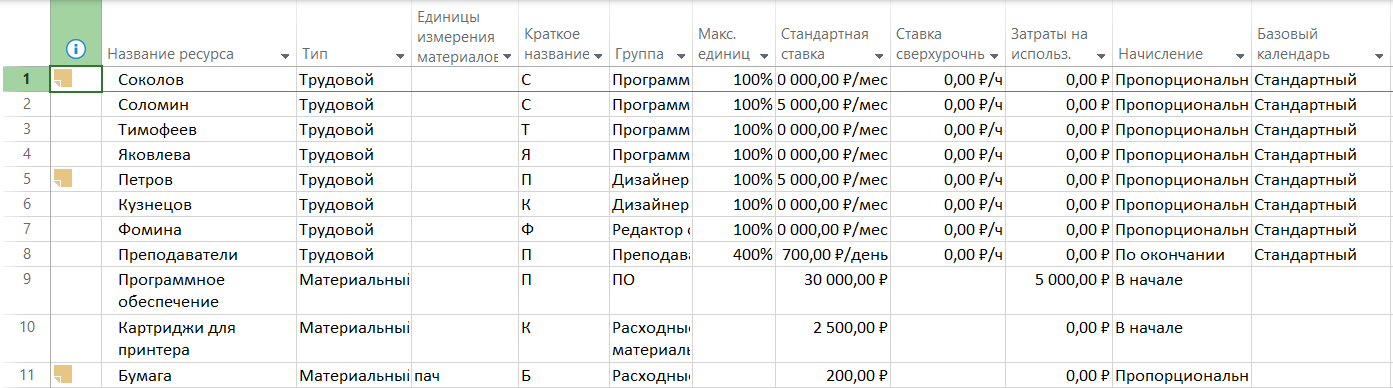
\includegraphics[width=\linewidth]{images/2.png}
	\caption{Список ресурсов проекта}
	\label{fig:2}
\end{figure}

\section{Задание 6}

Задачам были назначены ресурсы по варианту. Задачам 5 и 6 назначены фиксированные затраты 500 рублей, задаче 10~---~1000 рублей. Расход бумаги был установлен 3 пачки в месяц. После назначения ресурсов длительность проекта составила 56 дней, планируемая дата окончания 26.06, трудозатраты 1824 часа, затраты 623 450 рублей, что отображено на рисунке~\ref{fig:3}. Возникла перегрузка у сотрудников Кузнецова и Тимофеева, в связи с параллельным выполнением работ по разработке представительских сайтов.

\begin{figure}[H]
	\centering
	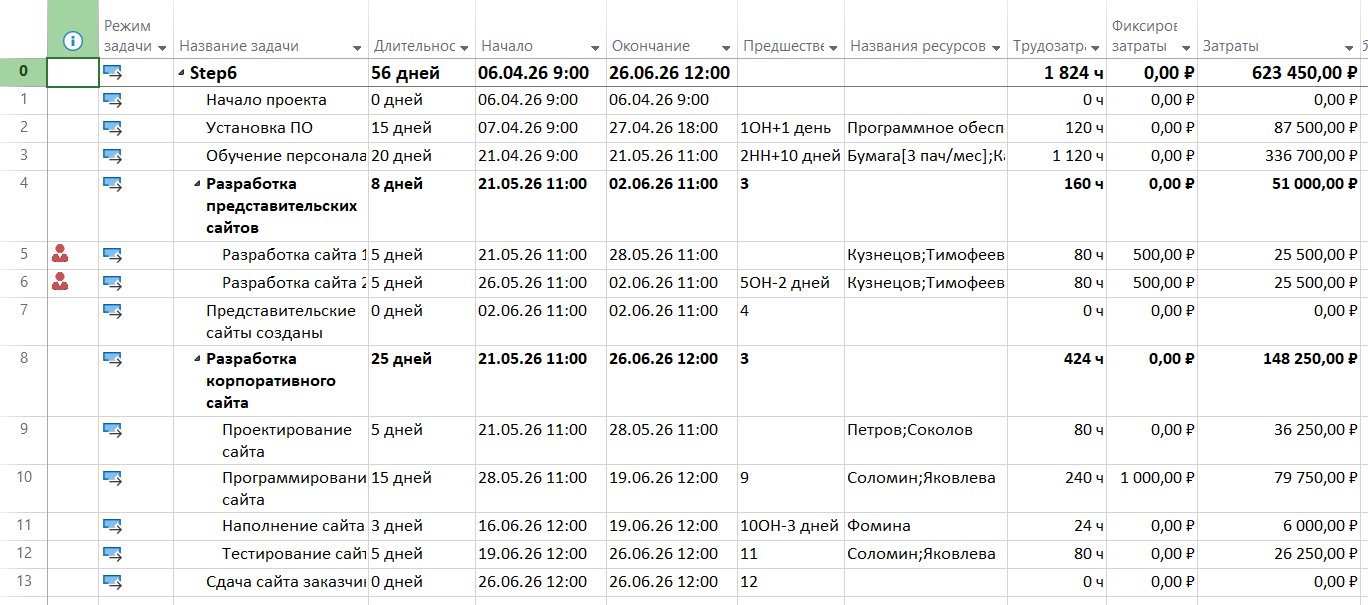
\includegraphics[width=\linewidth]{images/3.png}
	\caption{Назначение ресурсов задачам проекта}
	\label{fig:3}
\end{figure}

\section{Задание 7}

Задачи по разработке представительских сайтов разбиты на подзадачи по разработке дизайна (2 дня) и непосрественно программирование сайта (3 дня). Связи задач были обновлены. Разбиение помогло разрешить перегрузки сотрудников, что отображено на рисунке~\ref{fig:4}. Трудозатраты снизились до 1744 часов, затраты до 598 450 рублей, в связи с уменьшением времени работы  Кузнецовым и Тимофеевым с 10 до 4 и 6 дней соответственно.

\begin{figure}[H]
	\centering
	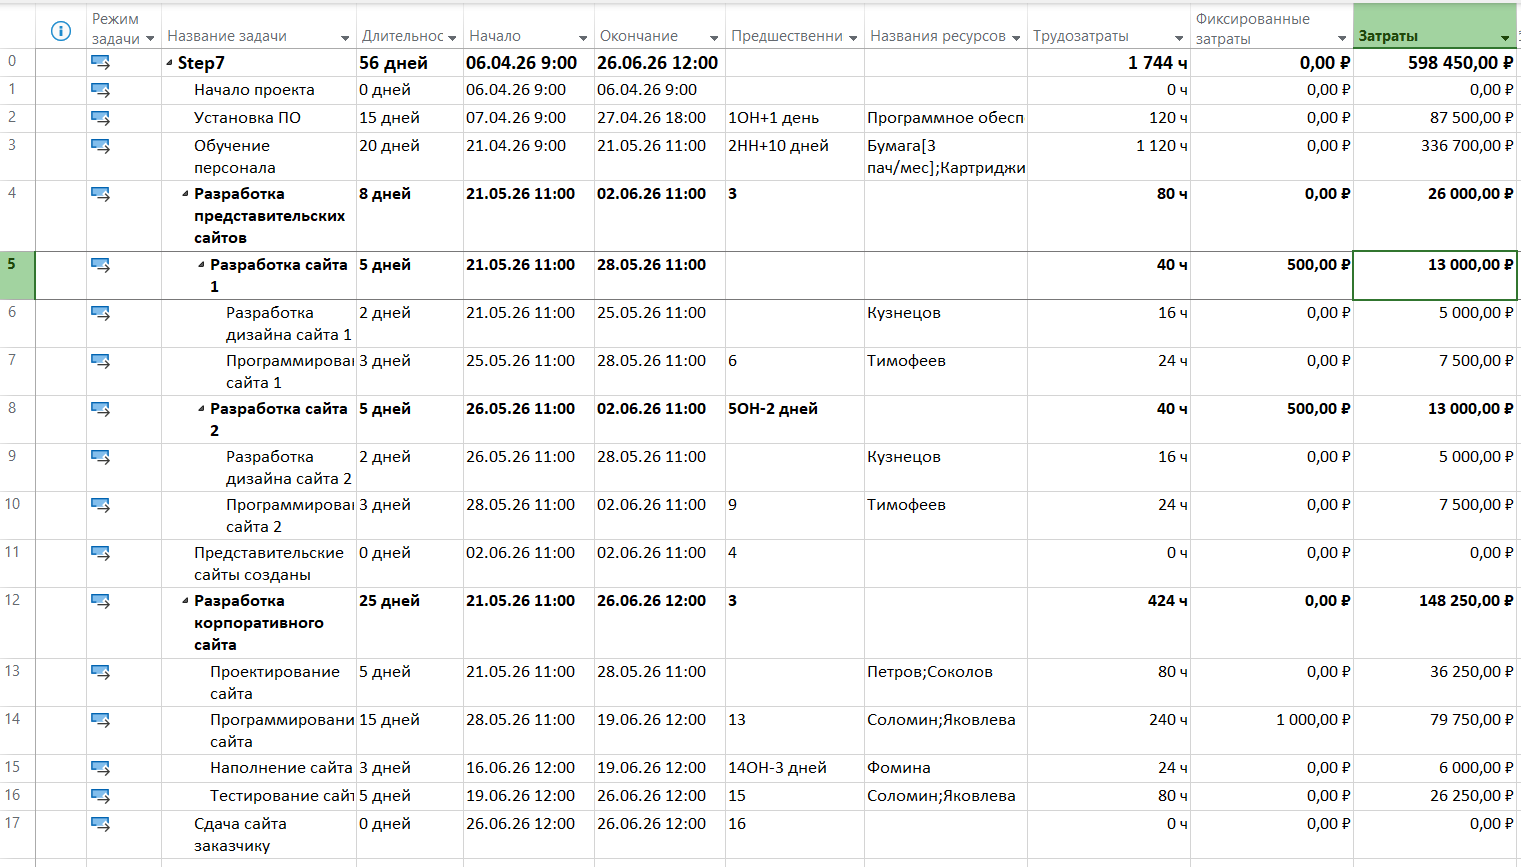
\includegraphics[width=\linewidth]{images/4.png}
	\caption{Разбиение задач 5 и 6 на подзадачи}
	\label{fig:4}
\end{figure}

\section{Задание 8}

При назначении Соколова на задачу обучения сотрудников и снижения числа единиц ресурса Преподаватели до 3 человек, длительность выполнения задачи снижается до 17.5 дней. Поскольку данная задача лежит на критическом пути планируемая дата окончания проекта также сдвигается на 23.06, однако увеличиваются затра до 617 925 рублей и возникают перегрузки по данному сотруднику.

\begin{figure}[H]
	\centering
	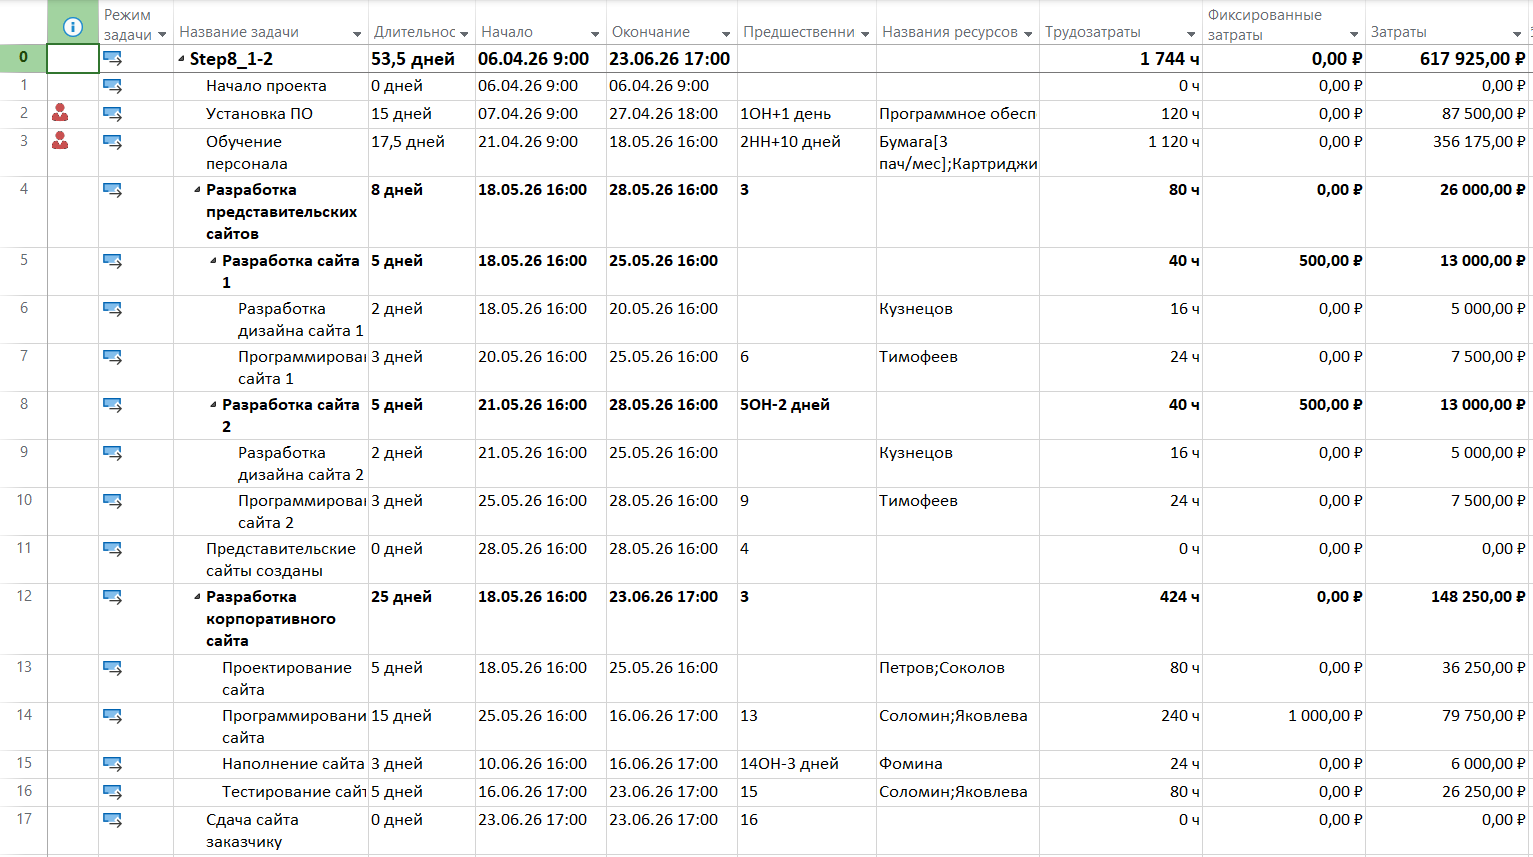
\includegraphics[width=\linewidth]{images/5.png}
	\caption{Назначение Соколова на задачу обучения сотрудников}
	\label{fig:5}
\end{figure}

\subsection{Вариант 1}

Для разрешения перегрузки по сотруднику Соколову, может быть установлена задержка его подключения к задаче обучения до момента окончания работ над задачей по установке ПО. В этом случае дата окончания задачи сдвигается на 25.05, вследствие чего сдвигается и дата окончания проекта на 30.06. Трудозатраты и затраты остаются неизменными. 

\begin{figure}[H]
	\centering
	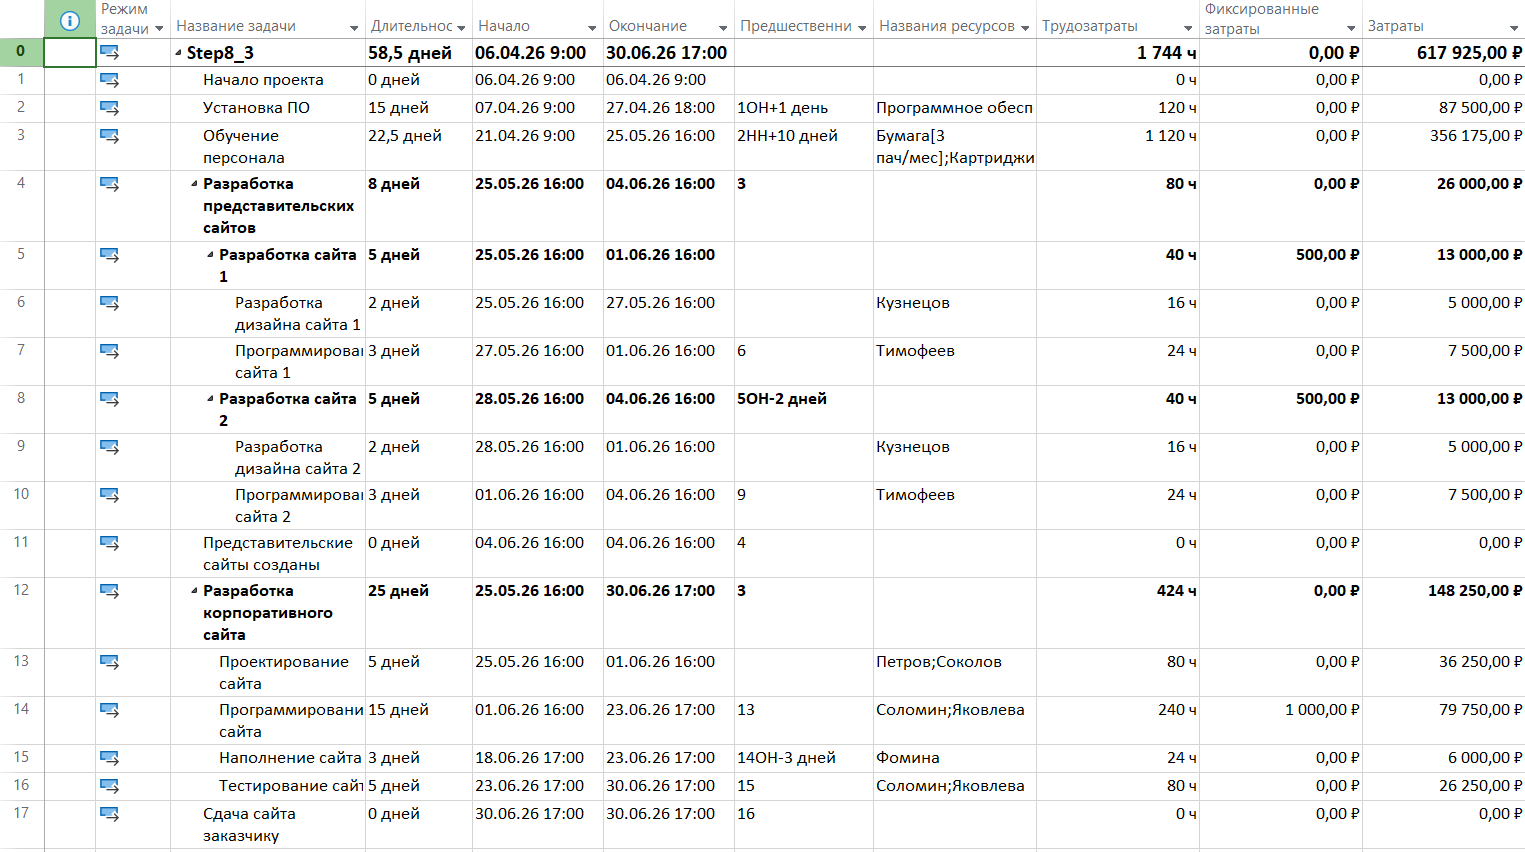
\includegraphics[width=\linewidth]{images/6.png}
	\caption{Изменение плана проекта при установки задержки для Соколова}
	\label{fig:6}
\end{figure}

\subsection{Вариант 2}

Другим подходом к разрешению перегрузки по сотруднику Соколову является варьирование профилей нагрузки данного сотрудника на задачах по установке ПО и обучению сотрудников. К разрешению перегрузки ведут комбинации профилей <<Загрузка в начале>>~---~<<Загрузка в конце>> и <<Загрузка в начале>>~---~<<Поздний пик>> по данным задачам.

В первом случае окончание задачи по обучению персонала смещается на 03.06, что ведет к смещению окончания проекта на 09.07, что является превышением допустимого срока в 3 месяца. Результаты на рисунке~\ref{fig:7}. Также увеличилась длительность работы над задачей установки ПО до 25 дней.

\begin{figure}[H]
	\centering
	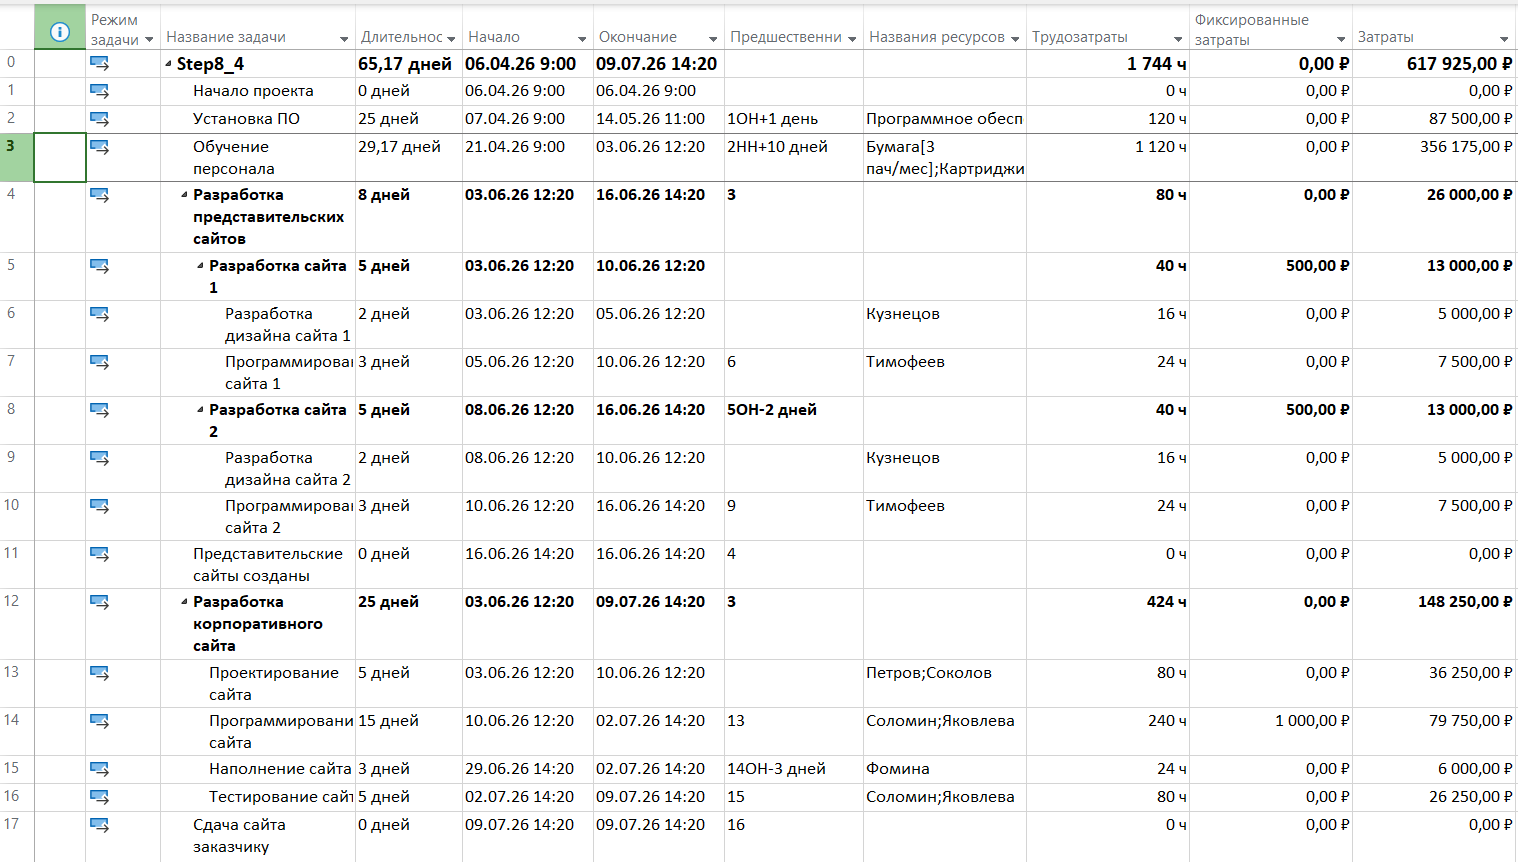
\includegraphics[width=\linewidth]{images/7.png}
	\caption{Использование профилей <<Загрузка в начале>>~---~<<Загрузка в конце>> для разрешения перегрузки Соколова}
	\label{fig:7}
\end{figure}

Во втором случае сроки выполенния задачи сдвигаются еще дальше на 11.06 и, как результат, также сдвигаются сроки выполнения проекта на 17.07, что также является превышением допустимых сроков выполнения проекта. Аналогично увеличилась длительность работы над задачей установки ПО до 25 дней.

\begin{figure}[H]
	\centering
	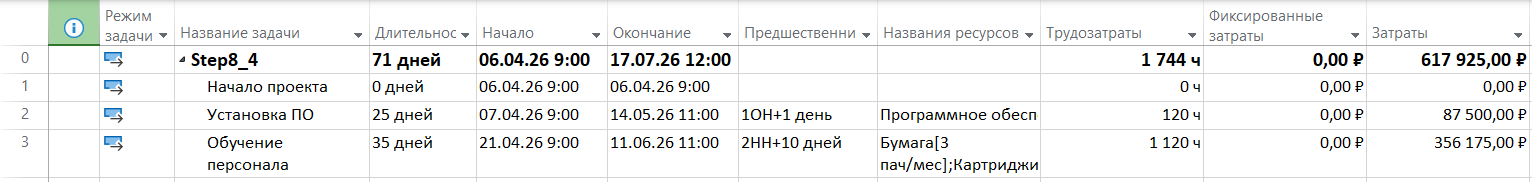
\includegraphics[width=\linewidth]{images/8.png}
	\caption{Использование профилей <<Загрузка в начале>>~---~<<Поздний пик>> для разрешения перегрузки Соколова}
	\label{fig:8}
\end{figure}

\subsection{Выводы}

Наиболее оптимальным способом разрешения перегрузки сотрудника Соколова является установка задержки для начала работ над задачей обучения сотрудников после окончания работ по задаче установки ПО, так как не ведет к превышению сроков проекта, однако сдвигает их на 2.5 дня. Привлечение Соколова к задаче обучения сотрудников при условии его единоличной работы над задачей по установке ПО не является оправданным, так как возрастают затраты и длительность работы над проектом. При этом в случае добавления сотрудников к задаче установки ПО и сокращении сроков работы над ней может привести к целесообразности добавления Соколова к задаче обучения сотрудников для сокращения времени ее выполнения.

\section{Задание 9}

Для сокращения длительности критического пути и, как следствие, длительности работы над проектом были применены следующие меры:
\begin{itemize}
	\item для задачи <<Установка ПО>> были дополнительно привлечены сотрудники Тимофеев и Яковлева, что позволило сократить длительность работ до 5 дней, затраты до 77 500 (-10 000) рублей;
	\item в связи с отсутствием пересечения задач по установке ПО и обучения сотрудников, Соколов был привлечен к задаче обучения сотрудников при количестве преподавателей~---~3, что позволило сократить длительность работ над задачей до 17.5 дней, однако возрасли затраты до 356 525 (+19 825) рублей;
	\item к задаче тестирования сайта был дополнительно подключен Тимофеев, что позволило сократить длительность выполнения до 3.33 дней и затраты до 25 833 (-727) рублей;
	\item в связи с занятостью Тимофеева на задачах по программированию представительских сайтов, он не может быть назначен на задачу программирования корпоративного сайта без возникновения перегрузок и удлинения критического пути, вследствие их устранения;
	\item Кузнецов мог бы быть назначен на задачу наполнения сайта, для сокращения длительности работ над ним, при условии обладания им необходимыми компетенциями.
\end{itemize}

В результате принятых мер, планируемая дата окончания проекта 22.06, что на две недели меньше максимально возможного срока, затраты составляют 607 858 рублей, что на 42 142 рублей меньше максимального бюджета проекта. Результаты приведены на рисунке~\ref{fig:9}.

\begin{figure}[H]
	\centering
	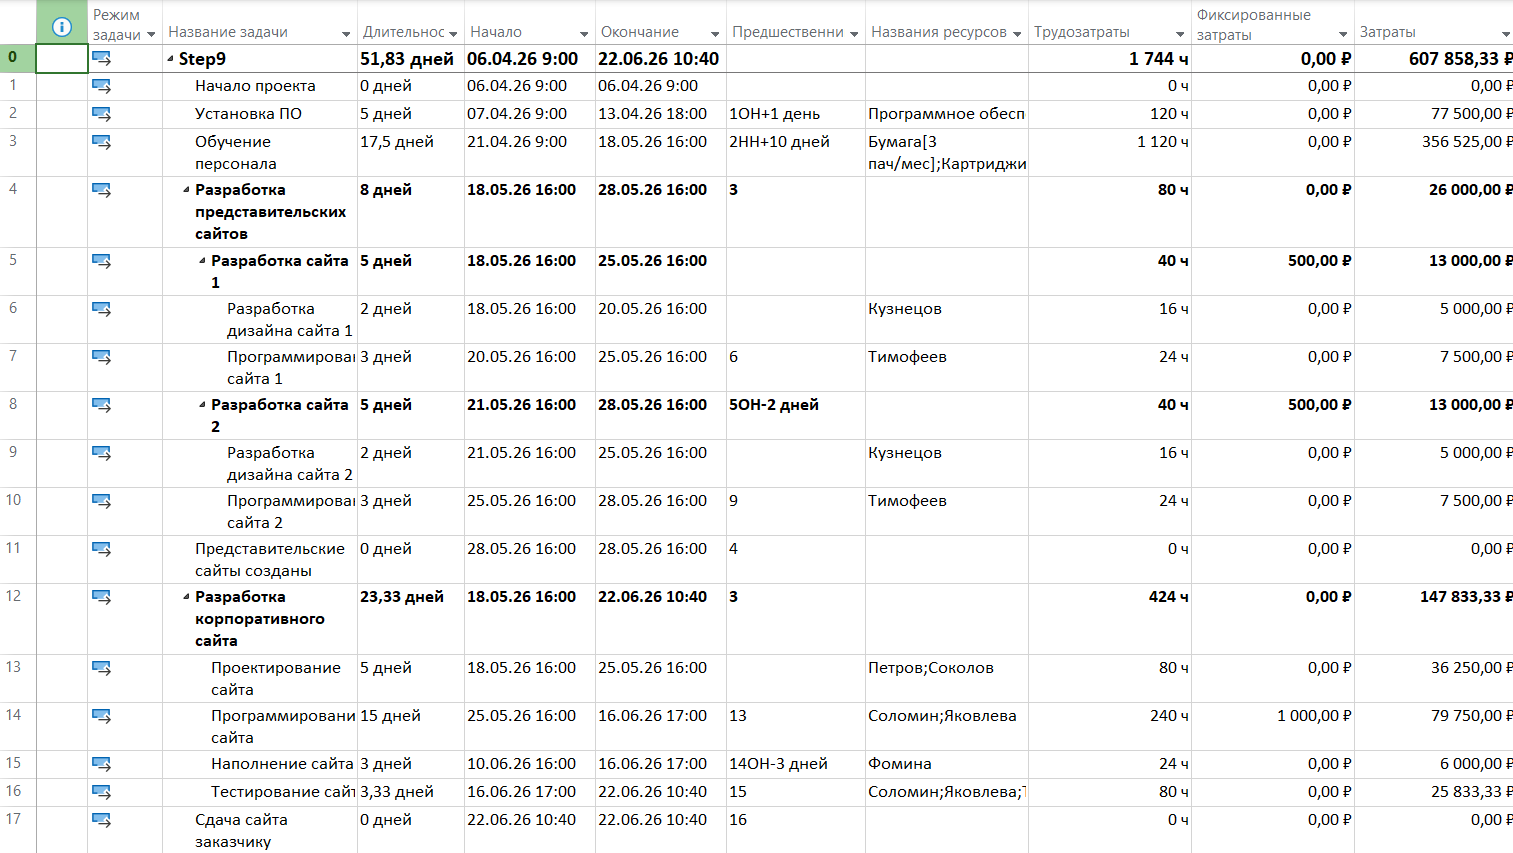
\includegraphics[width=\linewidth]{images/9.png}
	\caption{Сокращение критического пути}
	\label{fig:9}
\end{figure}

\section{Задание 10}

Дата отчета установлена 28.05 для отслеживания окончания работы над представительскими сайтами и полноценного переключения на работу с корпоративным сайтом. Для задач разработки дизайна и программирования сайта 2 установлено запаздывание окончания работ в 2 дня. Задачи 1--13, за исключением задач 4 и 10 отмечены выполеннными. Прогресс работы над задачей 10 составляет 60\%.

\begin{figure}[H]
	\centering
	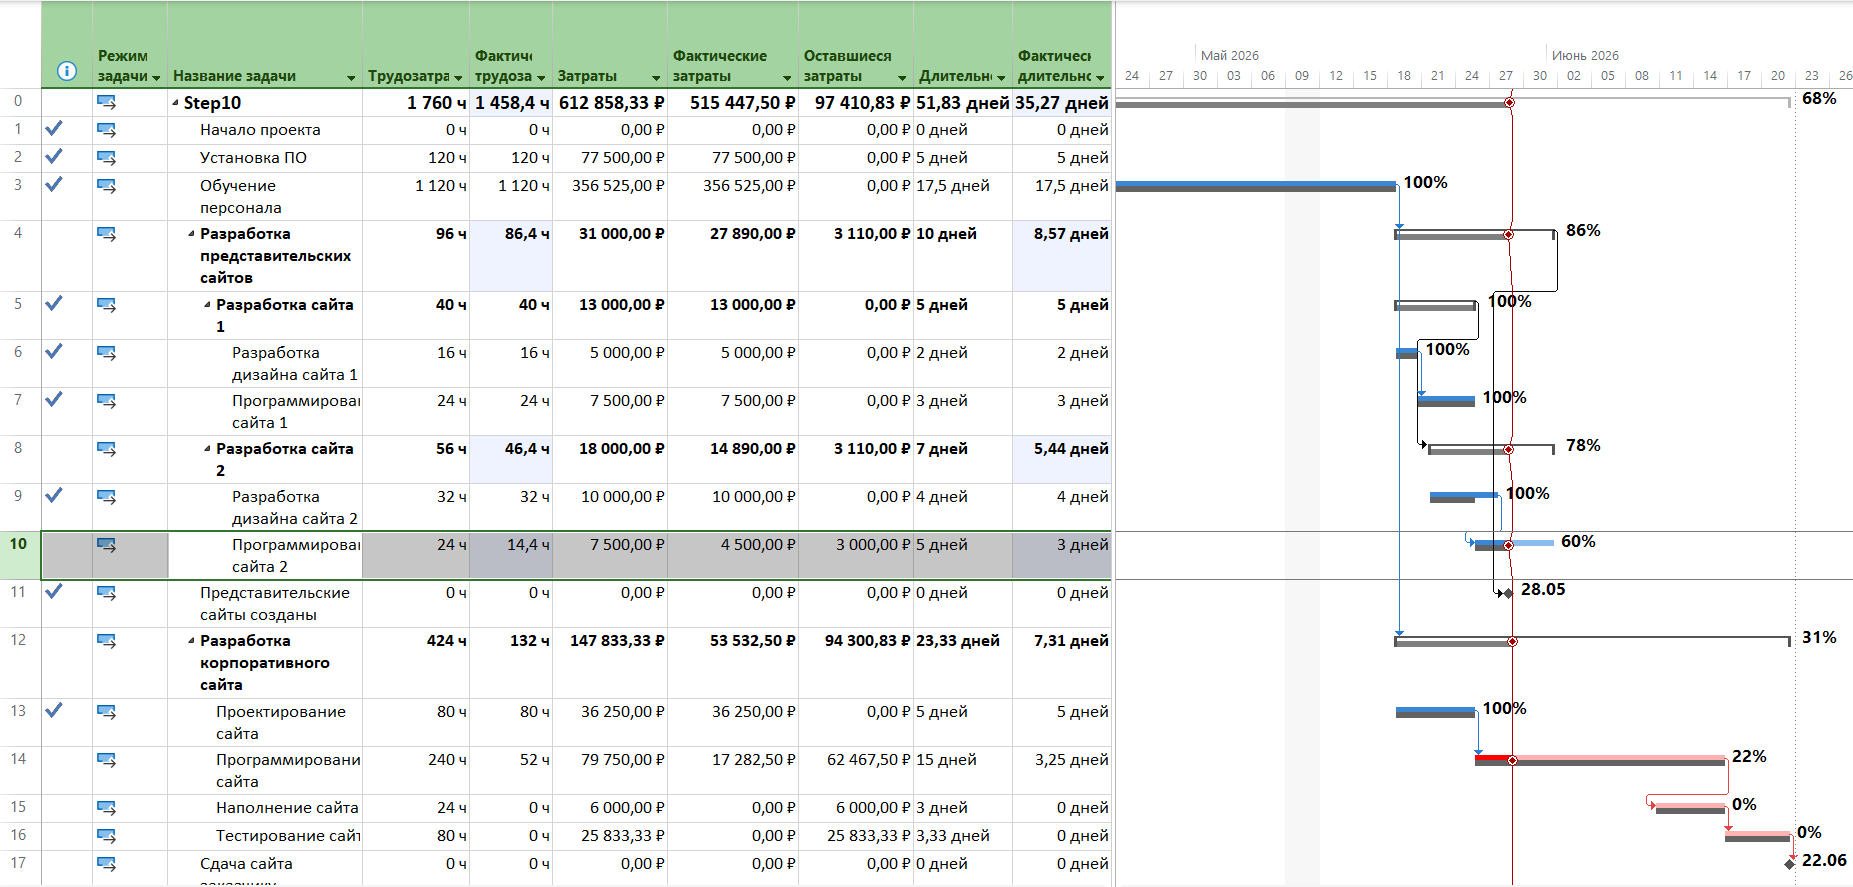
\includegraphics[width=\linewidth]{images/10.png}
	\caption{Диаграмма Ганта с отслеживанием и линией прогресса. Сравнение планируемых и фактических значений.}
	\label{fig:10}
\end{figure}

На 28.05 прошло 68\% длительности проекта. Потрачено 84\% планируемых затрат. Планируемые затраты в связи с задержками увеличились на 5000 рублей. Фактические трудозатраты составили 83\% планируемых.

\subsection*{Вывод}

Несмотря на задержки выполнения задач по разработке представительского сайта 2, сроки выполенния проекта остались прежними (22.06). В результате задержек затраты увеличились на 5000 рублей и на 28.05 составляют по плану 612 858 рублей. Запас по длительности по прежнему составляет 2 недели, по финансам~---~37 142 рубля.